\setbeamertemplate{caption}{\raggedright\insertcaption\par}
\captionsetup[figure]{labelformat=empty}% redefines the caption setup of the figures environment in the beamer class.

\frame{\frametitle{Fatigue damage}

 \uncover<1->{
  \twocol{	\begin{itemize}
    \item Fluctuating loads
   \end{itemize}
   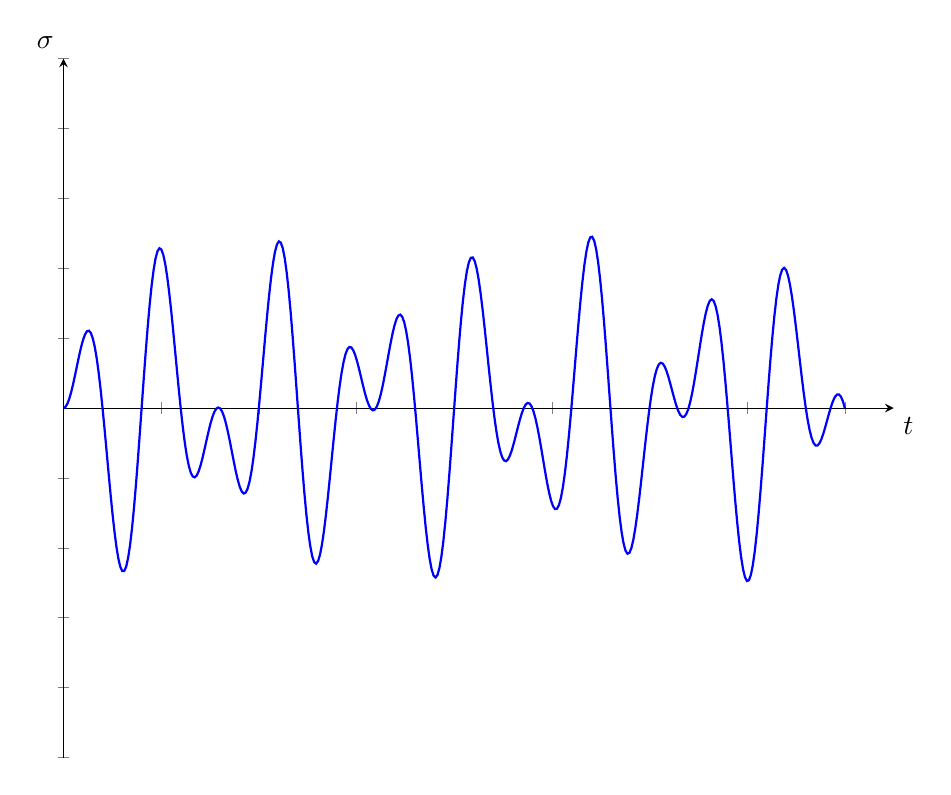
\begin{tikzpicture}[scale=1]
    \begin{axis}[axis x line=center, axis y line=center,
      xticklabels={},yticklabels={},xlabel style={below right},
      ylabel style={above left},ymin=-1,ymax=1,xmin=0,xmax=8.5,
      width=\textwidth,xlabel=$t$,ylabel=$\sigma$]
     \addplot [color=blue,thick,mark=none,domain=0:8,samples=400]{sin(2*\x r)*0.5*sin(pi / 2 * 5 * \x r)} ;
    \end{axis}
   \end{tikzpicture}
  }{
   \centering
   \uncover<2->{\hfil
    \begin{itemize}
     \item Material degradation\\[0.6cm]
    \end{itemize}

    \only<2>{\includegraphics[width=0.9\textwidth]{/home/alameddin/src/tex/templates/figures/windturbine.jpg}\\[-0.3cm]}

    \only<3->{\includegraphics[width=0.9\textwidth]{/home/alameddin/src/tex/templates/figures/bridge.jpg}\\[-0.3cm]}
    \uncover<2-3>{\vspace*{0.1cm} {\tiny Image by alegri / 4freephotos.com}}

   }

  }
 }
 {

 }
}



\frame{\frametitle{Fatigue damage}

 \twocol{	\begin{itemize}
   \item Fluctuating loads
  \end{itemize}
  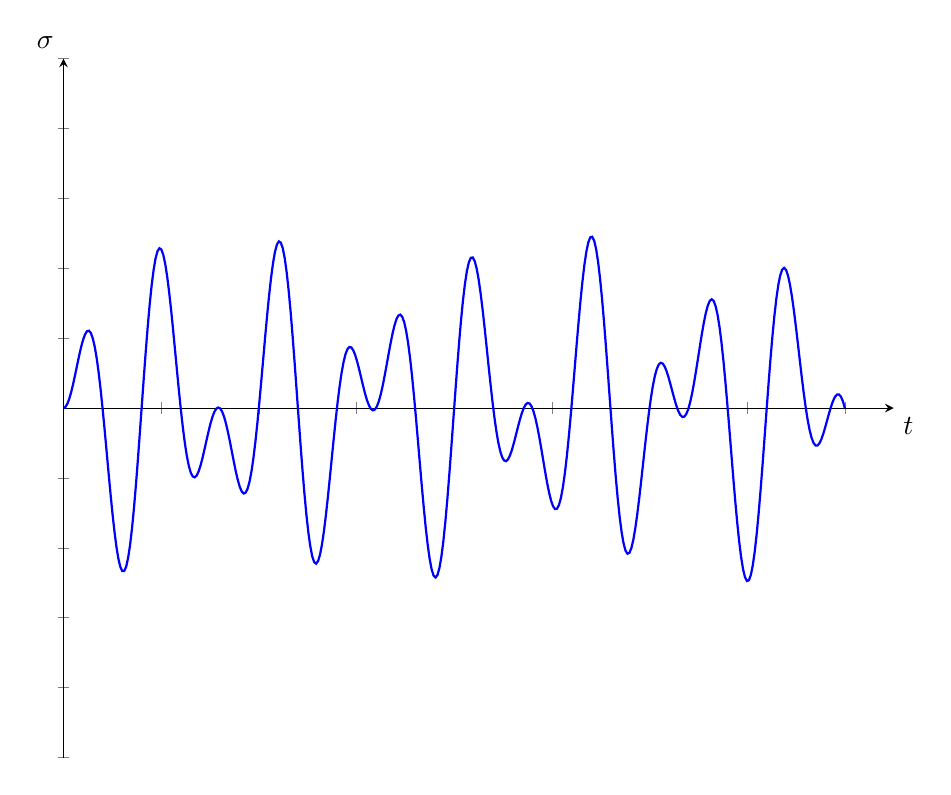
\begin{tikzpicture}[scale=1]
   \begin{axis}[axis x line=center, axis y line=center,
     xticklabels={},yticklabels={},xlabel style={below right},
     ylabel style={above left},ymin=-1,ymax=1,xmin=0,xmax=8.5,
     width=\textwidth,xlabel=$t$,ylabel=$\sigma$]
    \addplot [color=blue,thick,mark=none,domain=0:8,samples=400]{sin(2*\x r)*0.5*sin(pi / 2 * 5 * \x r)} ;
   \end{axis}
  \end{tikzpicture}
 }{
  \centering
  \uncover<1->{\hfil
   \uncover<1->{	\begin{itemize}
     {\item Virtual experiments\\[0.5cm]}
           {\item Continuum damage model\\[0.5cm]}
           {\item Millions of cycles\\[0.5cm]}
           {\item Macro crack initiation \\[0.5cm]}
           {\item Computationally expensive\\[0.5cm]}
    \end{itemize}}
  }
 }
 {
  \uncover<2>{
   \begin{block}{ \centering Model order reduction (MOR) techniques}
   \end{block}

  }
 }
}

\begin{frame}{Outline}
 \tableofcontents
\end{frame}

\section{State of art}
\begin{frame}{Outline}
 \tableofcontents[currentsection]
\end{frame}

\frame{\frametitle{ROM for non-linear problems}
 \begin{itemize}
  \item Short-term damage computations
        \begin{itemize}
         \footnotesize
         \item Proper orthogonal decomposition (POD)\\
               \qquad [Kerfriden et al, 2011-2012, Ryckelynck, 2005-2011].
         \item Proper generalised decomposition (PGD)\\
               \qquad [Bhattacharyya et al, 2017].
        \end{itemize}
        \vfill
  \item Long-term fatigue computations
        \begin{itemize}
         \footnotesize
         \item Temporal homogenisation \\ {\qquad [Fish and Yu, 2002; Devulder et al, 2010]}
         \item Space-time finite element method \\
               {\qquad[Oden, 1969; Bhamare, 2014; Fritzen and Hassani, 2018]}
         \item Modified jump cycle approach \\ {\qquad[Bhattacharyya et al, 2018]}
        \end{itemize}
 \end{itemize}
}

\frame{\frametitle{Previous works with LATIN}

 \begin{itemize}
  {\item \footnotesize An approach to include damage in a LATIN-PGD framework \dSmiley}
        {\item \footnotesize Modified jump cycle approach to tackle large number of cycles \dSmiley }
        \vfill
        {\item \footnotesize Limited to specific models and constant amplitude loads \frownie{}\\
  \item No two-time scale, no time savings and many modes are generated \frownie{}}
        \vfill
        {\item \footnotesize Generalised formulation for different nonlinear material models}
        {\item \footnotesize Efficient variable amplitude simulations}
 \end{itemize}
}


\section{Reduced order model for cyclic loading}
\begin{frame}{Outline}
 \tableofcontents[currentsection]
\end{frame}

\frame{\frametitle{Mechanical problem}
 \begin{block}{ \centering Admissibility equations}
 \end{block}
 \vspace{-0.5cm}
 \begin{minipage}[t]{0.4\textwidth}
  \begin{itemize}
   {\item Static admissibility }
         \vspace{-0.5cm}
         \begin{align*}
          \centering
          \div{\fsigma}+\fb & =\fzero \text{ \; in } \mathrm{\Omega}                                   \\
          \fsigma \cdot \fn & =\bar{\boldsymbol{t}} \text{\; \ on } \mathrm{\partial\Omega_\mathrm{N}}
         \end{align*}
  \end{itemize}
 \end{minipage}\hfil\begin{minipage}[t]{0.5\textwidth}
  \begin{itemize}
   {\item Kinematic admissibility}
         \vspace{-0.5cm}
         \begin{align*}
          \centering
          \feps & = \grads{u} \text{ \; in } \mathrm{\Omega}                        \\
          u     & =\bar{u} \quad \text{ \;  on } \mathrm{\partial\Omega_\mathrm{D}}
         \end{align*}
  \end{itemize}
 \end{minipage}

 \begin{block}{ \centering Nonlinear material model}
 \end{block}
 \vspace{-0.5cm}
 \begin{minipage}[t]{0.4\textwidth}
  \begin{itemize}
   {\item State equations}
         \centering
         \vspace{-0.3cm}
         \begin{equation*}
          \begin{split}
           \fsigma &=f({\psi,\fepse}) \\
           \fbeta &= g({\psi,\falpha})\\
           Y &=q({\psi,D})
          \end{split}
         \end{equation*}
  \end{itemize}
 \end{minipage}\hfil\begin{minipage}[t]{0.5\textwidth}
  \begin{itemize}
   {\item Evolution equations}
         \centering
         \vspace{-0.3cm}
         \begin{equation*}
          \begin{split}
           {\dot{\epst}}^{\rm p} &= \hat{f}({\phi,\sig})\\
           {\dot\alpha} &=\hat{g}({\phi,\beta}) \\
           {\dot{D}} &= \hat{q}({\phi,D})
          \end{split}
         \end{equation*}
  \end{itemize}
 \end{minipage}

}
\frame{\frametitle{Solution algorithm}
 \begin{itemize}
  {\item Many LATIN algorithms for different non-linear problems }
        {\item A combination with some modifications}
        \begin{itemize}
         {\item Local stage, given initial conditions }	\\
               \qquad Solve the state and evolution equations to get $\stepj[]{s}$
               {\item Global stage }\\
               \qquad Solve the admissibility equations to get $\stepk[]{s}$
               {\item Data flow between these stages}
               \vspace{-0.3cm}
               \begin{equation*}
                \begin{split}
                 (\stepj[]{\fsigma}-\stepi[]{\fsigma}) \; +  {\ffH^+} \ \; (\stepj[]{\feps}-\stepi[]{\feps}) \ \; &=\fzero\\
                 (\stepk[ ]{\fsigma}-\stepj[ ]{\fsigma}) -{\ffH^-}(\stepk[]{\feps}-\stepj[]{\feps})&= \fzero
                \end{split}
               \end{equation*}
         \item Iterate until convergence with an energy error indicator
               \begin{align*}
                \footnotesize
                \xi =\frac{\normg{\stepk[]{s}-\stepj[]{s}}{}}{\frac{1}{2} \normg{\stepk[]{s} + \stepj[]{s}}{} }{} , \qquad
                \normg{s}{}^2 = \intspt (\fsigma:\ffC^{-1} \fsigma + \feps:\ffC \ \feps ) \ \d \Omega \d t
               \end{align*}
        \end{itemize}
 \end{itemize}
}

\frame{\frametitle{The global stage}
 \begin{itemize}
  \item Weak form at iteration $i+1$
        \begin{equation*}
         \hspace{-0.5cm} \footnotesize \intspt \stepk[]{\fsigma}:\feps(\su) \dspt = \intspt \fb \cdot \su  \d \Omega \d t+ \intt{\pOmegaN}  \bar{\ft} \cdot \su \d S \d t, \quad \forall \su \in \cal{U}_{\mathrm{0}}
        \end{equation*}
        \vfill
  \item Correction $\Delta\stepk[]{\bullet}=\stepk[]{\bullet}-\stepi[]{\bullet}$
        \begin{align*}
                 & \Delta\stepk[]{\fsigma} - {\ffH^-} \Delta\stepk[]{\feps} - \hf=\fzero, \ \  \hf  = \underbrace{(\stepj{\fsigma}-\stepi{\fsigma}) - {\ffH^-} (\stepj[]{\feps}-\stepi[]{\feps})}_{known} \\
         \intspt & \Delta \stepk[]{\fsigma} : \feps(\Delta \su) \ \d \Omega \d t = 0
        \end{align*}
 \end{itemize}
}

\frame{\frametitle{Proper Generalised Decomposition}
 \begin{itemize}
  \item  Low-rank approximation of the solution
        \begin{equation*}
         {u}(\fx,t)=\ds \sum_{i=1}^{N} \lambda_i(t) \ v_i(\fx)
        \end{equation*}
  \item  Enriching with one mode
        \begin{align*}
         \Delta u = \lambda(t) \ v(\fx) \qquad \Delta u^\ast = \lambda^\ast \ v + \lambda \ v^\ast
        \end{align*}
  \item Updating $(\mu)$ previously generated time modes
        \begin{align*}
         \Delta u = \ds \sum_{i=1}^{\mu} \Delta \lambda_i(t) \ \underbrace{v_i(\fx)}_{known}
        \end{align*}
 \end{itemize}
}

\frame{\frametitle{Static admissibility}
 \footnotesize
 \begin{itemize}
  \item  Static admissibility and global search direction
        \footnotesize{\begin{align*}
          \intspt  {\ffH^-} \Delta\stepk[]{\feps}  : \feps(\Delta \su) \ \d \Omega \d t & = - \intspt \hf : \feps(\Delta \su) \ \d \Omega \d t
         \end{align*}}
  \item Space problem: {\footnotesize $ \tiny \vol{\bullet} = \intT \bullet \ \d t$}, given $\lambda_j$
        \footnotesize{
         \begin{align*}
          \vol{\lambda_j \lambda_j} \intS \grad{v}^\ast  : {\ffH^-}  \grad{v_{j+1}} \ \d \Omega & = - \vol{\lambda_j} \intS \grad{v}^\ast : \hf \d \Omega
         \end{align*}}
        \vspace{-0.2cm}
  \item Time problem, given $v_{j+1}$:
        \begin{align*}
         \footnotesize
         \intT \lambda^\ast \left[ \intS  \grad{v_{j+1}} : {\ffH^-} \ \grad{v_{j+1}} \d \Omega \right] \lambda_{j+1} \ \d t & = - \vol{\lambda^\ast} \intS  \grad{v_{j+1}} : \hf \d \Omega
        \end{align*}
 \end{itemize}
 %		\mediabutton[jsaction={anim.myAnim.playFwd();}]{\fbox{\strut Play}}
 %		\mediabutton[jsaction={anim.myAnim.pause();}]{\fbox{\strut Pause}}
 %		 \includegraphics[width=0.4\linewidth]{./img/lating-0.png}
}

\frame{\frametitle{Algorithmic point of view}
 \begin{itemize}
  \item Choosing the search directions as
        \begin{equation*}
         \footnotesize
         {\ffH^+} = 0, \qquad {\ffH^-} = \alpha \ \ffC \qquad \alpha \in \ ]0,1]
        \end{equation*}
  \item Enrichment
        \begin{equation*}
         \begin{split}
          \gamma \ \mK \ \vec{v}_{i+1} &= \vec{F} \qquad \ \gamma \in \ffR \qquad \mK \in \ffR^{n \times n} \qquad \vec{F} \in \ffR^{n} \\
          a \ \vlambda_{i+1} &= \vb  \qquad \ \ \, a \in \ffR \qquad  \ \, b \in \ffR^{n_t}
         \end{split}
        \end{equation*}
  \item Update\vspace{-0.2cm}
        \begin{equation*}
         \begin{split}
          \hspace{-1cm} \mA \ \{\Delta \vlambda_i\} = \mat{b}  \qquad \ \mA \in \ffR^{N \times N} \qquad \mat{b} \in \ffR^{N \times n_t}
         \end{split}
        \end{equation*}
 \end{itemize}
}

\frame{\frametitle{Multiple cycles with variable load amplitudes}
 \begin{itemize}
  \item The stiffness\\
        \uncover<2>{\qquad Computed only once\\}
        \vfill
  \item The elastic solution\\
        \uncover<2>{\qquad Only once and parametrised over the load amplitude\\}
        \vfill
  \item An initial guess\\
        \uncover<2>{\qquad From the previous cycle\\}
 \end{itemize}
}

\frame{\frametitle{The initial guess}
 \begin{itemize}
  \item Time modes are shifted and scaled to ensure continuity\\
        \begin{figure}
         \hspace{-1.5cm}\vspace{1cm}
         \centering
         \includegraphics[width=0.6\linewidth]{/home/alameddin/src/tex/templates/tex_figures/cyclic_shift.pdf}
        \end{figure}
        \vspace{-2cm}
        \begin{align*}
         \qquad \lambda_2(t) & = \lambda_1(t) + a \ t + b                                       \\
         \lambda_2(\tau_1)   & = \lambda_2(\tau_1) \qquad \lambda_2(\tau_2) = \lambda_2(\tau_1)
        \end{align*}
 \end{itemize}
}

\section{Numerical examples}

\begin{frame}{Outline}
 \tableofcontents[currentsection]
\end{frame}

\frame{\frametitle{Numerical results}
 \begin{itemize}
  \item A plate with a central groove subjected to cyclic loading\\ (Cr-Mo steel at $20^\circ \rm C$ and $580^\circ \rm C$)
        \begin{figure}
         \centering
         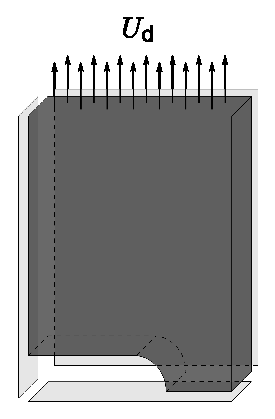
\includegraphics[scale=0.7,clip]{/home/alameddin/src/tex/templates/figures/3d_plate_1_8.eps}
        \end{figure}
 \end{itemize}
}

\frame{\frametitle{Quasi-brittle material model}
 In collaboration with Bhattacharyya and Desmorat\\
 \begin{itemize}
  \item Two-scale damage model
        \vspace{-0.5cm}
        \begin{figure}
         \centering
         \includegraphics[scale=0.60,clip]{/home/alameddin/src/tex/templates/figures/two_length_scale.eps}
        \end{figure}
  \item With an adaptive jump cycle algorithm
 \end{itemize}
}

\frame{\frametitle{Damage evolution}
 \begin{figure}
  \centering
  \includegraphics[width=0.5\linewidth]{/home/alameddin/src/tex/templates/figures/D_3d.eps}
  \caption{\qquad \qquad Damage evolution at the weakest Gauss point}
 \end{figure}
}

\frame{\frametitle{Damage behaviour}
 \vspace{2cm}
 \twocol{
  \begin{figure}
   \centering
   \includegraphics[width=0.85\linewidth,clip]{/home/alameddin/src/tex/templates/figures/damage_micro.eps}
   \caption{\qquad \qquad Damage distribution\\ \qquad \qquad \ \ at the micro-scale}
  \end{figure}}
 {\begin{figure}
   \includegraphics[width=0.9\linewidth]{/home/alameddin/src/tex/templates/figures/D_mac_phi.eps}
   \caption{\hspace{-0.4cm} $D=1-(1-D^\mu)^\Phi$}
  \end{figure}
 }{}}


\frame{\frametitle{Visco-plastic material model}

 \begin{minipage}[t]{0.4\textwidth}
  \begin{itemize}
   {\item State equations}
         \vspace{-0.3cm}
         \begin{equation*}
          \begin{split}
           \fsigma & = \ffC \ \fepse \ (1-D) \\
           \fbeta &= C \ \falpha \\
           Y & = \frac{1}{2} \fepse : \ffC \ \fepse
          \end{split}
         \end{equation*}
  \end{itemize}
 \end{minipage}\hfil\begin{minipage}[t]{0.5\textwidth}
  \begin{itemize}
   {\item Evolution equations}
         \vspace{-0.3cm}
         \small
         \begin{equation*}
          \begin{split}
           {\dot{\epst}}^{\rm p} &=  k \ \vol{\Fp}_+^{n} \ \left[\frac{3}{2} \frac{\ftau}{J_{2}(\ftau)} \right] \frac{1}{1-D}\\
           {\dot\alpha} &= k \ \vol{\Fp}_+^{n} \ \left[ \frac{3}{2} \frac{\ftau}{J_{2}(\ftau)} - \frac{a}{C} \fbeta \right] \\
           {\dot{D}} &=  \kd  \vol{\Fd}_+^{\nd}
          \end{split}
         \end{equation*}
  \end{itemize}
 \end{minipage}
 \vspace{0.5cm}

}


\frame{\frametitle{Variable amplitude}
 \twocol{\begin{figure}
   \centering
   \vspace{1cm}
   \includegraphics[width=0.9\textwidth]{/home/alameddin/src/tex/templates/tex_figures/variable_load_12cycles.pdf}
  \end{figure}}{\begin{figure}
   \centering
   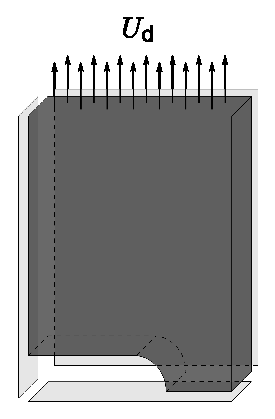
\includegraphics[scale=0.7,clip]{/home/alameddin/src/tex/templates/figures/3d_plate_1_8.eps}
  \end{figure}}{ }
}

\frame{\frametitle{Variable amplitude}
 \vspace{1.5cm}
 \twocol{\begin{figure}
   \includegraphics[width=0.9\linewidth]{/home/alameddin/src/tex/templates/tex_figures/damage_12cycles.pdf}
   %		\caption{Damage w.r.t. number of cycles}
   \label{fig_damage_evolution12cycles}
  \end{figure}}{\begin{figure}
   \includegraphics[width=0.9\linewidth]{/home/alameddin/src/tex/templates/tex_figures/number_pgdmodes_12cycles.pdf}
   %		\caption{Number of PGD modes in each cycle}
   \label{fig_pgdmodes12cycles}
  \end{figure}}{}
}

\frame{\frametitle{Variable amplitude}
 \vspace{1.5cm}
 \twocol{\begin{figure}
   \includegraphics[width=0.82\linewidth]{/home/alameddin/src/tex/templates/tex_figures/iterations_12cycles.pdf}
   %	\caption{Number of iteration}
  \end{figure}}{\begin{figure}
   \includegraphics[width=1\linewidth]{/home/alameddin/src/tex/templates/tex_figures/error_12cycles.pdf}
   %	\caption{Error indicator}
   \label{fig_err_12cycles}
  \end{figure}}{}
}

% \frame{\frametitle{Overloads}
%  \vspace{0.8cm}
%  {\begin{figure}
%    \centering
%    \includegraphics[width=0.6\linewidth]{/home/alameddin/src/tex/templates/tex_figures/overload.pdf}
%   \end{figure}}
% }

\frame{\frametitle{Random amplitudes}
 Cyclic load with the random amplitudes\\[0.2cm]
 % \vspace{0.2cm}
 \only<1>{\begin{figure}
   \centering
   \includegraphics[width=0.6\linewidth]{/home/alameddin/src/tex/templates/tex_figures/randomload0.pdf}
  \end{figure}}
 \only<2>{\begin{figure}
   \centering
   \includegraphics[width=0.6\linewidth]{/home/alameddin/src/tex/templates/tex_figures/randomload1.pdf}
  \end{figure}}
 \uncover<3->{\begin{figure}
   \centering
   \includegraphics[width=0.6\linewidth]{/home/alameddin/src/tex/templates/tex_figures/randomload_damage.pdf}
  \end{figure}}
 \uncover<4>{\begin{block}{ \centering Number of modes is less than 20}
  \end{block}}
}

\section{Conclusions and future research}
\begin{frame}{Outline}
 \tableofcontents[currentsection]
\end{frame}

\frame{\frametitle{Conclusion and future research}
 \vspace{0.5cm}
 \begin{itemize}
  \item Efficient cycle by cycle simulation for damage problems.
  \item Works for low and high cycle fatigue.\\[0.3cm]
        \vfill
        \pause
        \textbf{Challenges}
  \item \ The computation of the local stage.
  \item \ The integration of the error indicator and the time update.\\[0.3cm]
        \vfill
        \pause
        \textbf{Future development}
  \item Machine learning in the local stage.
  \item Reduced integration scheme.
 \end{itemize}
 \pause
 {\begin{block}{ \centering Thank you for your attention}
  \end{block}}
}

\frame{\frametitle{Github repository}
 \centering https://github.com/dbeurle/neon
}

\frame{\frametitle{Quasi-brittle material model}
Eshelby-Kr\"{o}ner localisation law
\begin{equation*}
 \label{twr}
 \left( \bm{\varepsilon}^{\mu}-\bm{\varepsilon}\right)  =  \gamma \left(  \bm{\varepsilon}^{\mu,p}-\bm{\varepsilon}^{p}\right) ,
\end{equation*}

where $\gamma$ is the Eshelby coefficient given by
\begin{equation*}
 \gamma = \dfrac{2}{15}\dfrac{4-5\nu}{1-\nu}.
\end{equation*}
}
\frame{\frametitle{Quasi-brittle material model}
 \begin{minipage}[t]{0.4\textwidth}
  \begin{itemize}
   {\item State equations}
         \vspace{-0.3cm}
         \begin{align*}
           & \tilde{\bm{\sigma}}^{\mu}= \bm{\mathrm{C}} \bm{\varepsilon}^{\mu,e}   & \\
           & Y^{\mu}=R_{v}\dfrac{\left( \tilde{\sigma}^{\mu}_{eq}\right) ^{2}}{2E}   \\
           & \bm{\beta}^{\mu}=\bm{\mathrm{Q}}\bm{\alpha}^{\mu}                     &
         \end{align*}
  \end{itemize}
 \end{minipage}\hfil\begin{minipage}[t]{0.5\textwidth}
  \begin{itemize}
   {\item Evolution equations}
         \vspace{-0.3cm}
         \small
         \begin{align*}
           & \dot{\bm{\varepsilon}}^{\mu,p} =  \dfrac{3}{2} \dfrac{\tilde{\bm{\sigma}}^{\mu} - \bm{\beta}^{\mu}}{\left( \tilde{\bm{\sigma}}^{\mu} - \bm{\beta}^{\mu} \right)_{eq}}  \dfrac{\dot{\lambda}_p}{1-D^{\mu}} & \\
           & \dot{\bm{\alpha}}^{\mu}=\dfrac{3}{2} \dfrac{\tilde{\bm{\sigma}}^{\mu} - \bm{\beta}^{\mu}}{\left( \tilde{\bm{\sigma}}^{\mu} - \bm{\beta}^{\mu} \right)_{eq}} \dot{\lambda}_p                               & \\
           & \dot{D}^{\mu} = \left( \dfrac{Y^{\mu}}{S} \dot{p}^{\mu} \right)^{s}                                                                                                                                       &
         \end{align*}
  \end{itemize}
 \end{minipage}
}

\frame{\frametitle{Crack closure effect}
 The effective stress
 \begin{equation*}
  \tilde{\bm{\sigma}} = \dfrac{\bm{\sigma}_{D}}{1-D} +
  \left[ \dfrac{\left\langle \sigma_{H}\right\rangle }{1-D}+ \left\langle -\sigma_{H}\right\rangle \right] \mathbb{I}
 \end{equation*}
 The triaxiality function
 \begin{align*}
  R_{v} = \dfrac{2}{3} \left( 1 + \nu\right) +3\left(1-2 \nu\right) \left\langle \dfrac{\sigma_{H}^{\mu}}{\sigma_{eq}^{\mu}} \right\rangle^{2} \\
  \sigma^{\mu}_{eq} = \sqrt{\dfrac{3}{2}\sigma^{\mu}_{D_{ij}} \sigma^{\mu}_{D_{ij}}} \qquad \tilde{\sigma}^{\mu}_{eq} = \sqrt{\dfrac{3}{2}\tilde{\sigma}^{\mu}_{D_{ij}} \tilde{\sigma}^{\mu}_{D_{ij}}}
 \end{align*}

 The micro-scale yield function $f^{\mu}$ is given as
 \begin{equation*}
  f^{\mu} = \left( \tilde{\bm{\sigma}}^{\mu}_{D} - \bm{\beta}^{\mu} \right) _{eq} - \sigma_f^{\infty},
 \end{equation*}
}

\frame{\frametitle{Stress-strain response}
 \begin{figure}[htbp!]
  \centering
  \includegraphics[width=0.8\linewidth,clip]{/home/alameddin/src/tex/templates/figures/stress_strain_micro.eps}
  \caption{Stress-strain diagram at certain cycles at the micro-scale}
 \end{figure}
}

\frame{\frametitle{Visco-plastic material model}
 \begin{itemize}
  \item Free energy function
        \begin{align*}
         \psi(\epse,\alpha,D) = \frac{1}{2} \fepse : \ffC (1-D) \ \fepse +  \frac{1}{2} \ C \ \falpha:\falpha
        \end{align*}
  \item Dissipation potential
        \begin{align*}
         \phi         & =\phip +\phid                                                                                            \\
         \phi^{\rm p} & = \frac{\kp}{\np+1} \vol{\Fp}_+^{\np+1}, \qquad \Fp= J_{2}(\ftau) + \frac{a}{2C} \ \fbeta:\fbeta - \sigy \\
         \phid        & = \frac{\kd}{\nd+1} \vol{\Fd}_+^{\nd+1}, \qquad \Fd=Y-Y_0                                                \\
        \end{align*}
 \end{itemize}
 \begin{equation*}
  \centering
  J_{2}(\ftau) = \sqrt{\frac{3}{2} \ftau:\ftau} \qquad \ftau=\frac{\fsigma^{\rm dev}}{(1-D)} - \fbeta
 \end{equation*}
}

\frame{\frametitle{Variable amplitude}
 \vspace{1.5cm}
 \twocol{\begin{figure}
   \includegraphics[width=0.9\linewidth]{/home/alameddin/src/tex/templates/figures/euromech/damage_12cycles.png}
   \caption{Damage distribution}
  \end{figure}}{\begin{figure}
   \includegraphics[width=0.9\linewidth]{/home/alameddin/src/tex/templates/figures/euromech/residual_vonmises_12cycles.png}
   \caption{Von Mises stress distribution}
  \end{figure}}{}
}

\frame{\frametitle{Numerical results}
 \twocol{\begin{figure}
   \includegraphics[width=0.9\linewidth]{/home/alameddin/src/tex/templates/figures/euromech/neon_damage.png}\\
   {Newton-Raphson}
  \end{figure}}{\begin{figure}
   \includegraphics[width=0.9\linewidth]{/home/alameddin/src/tex/templates/figures/euromech/latin_damage.png}\\
   \centering{LATIN-PGD}
  \end{figure}}{\centering
  \vspace{-1cm}
  Damage contour at the last time step\\
  \vfill
 }

}

\frame{\frametitle{Numerical results}
 \twocol{\begin{figure}
   \includegraphics[width=0.9\linewidth]{/home/alameddin/src/tex/templates/figures/euromech/neon_stress.png}\\
   {Newton-Raphson}
  \end{figure}}{\begin{figure}
   \includegraphics[width=0.9\linewidth]{/home/alameddin/src/tex/templates/figures/euromech/latin_stress.png}\\
   {LATIN-PGD}
  \end{figure}}{\centering
  \vspace{-1cm}
  Residual stress distribution after removing the load
 }
}

\frame{\frametitle{Differences}

 \begin{itemize}
  \item State equations in the local stage
  \item PGD for the strain instead of the plastic one
  \item Cycle by cycle
  \item Modes rescaling
 \end{itemize}

}

% 12 cycles
%main(linspace(33,66,12)*1e-4)

% random load
%r = ones(1,100) * 42e-4;
% r(4:6) = 52e-4;
%r(49:51) = 52e-4;
% r(94:96) = 52e-4;


https://github.com/dbeurle/neon
